% -*- coding: utf-8; -*-

\chapter{Introduction}
Why coq? Coq is a expressive functional programming language for writing formal proofs. It helps us reason about complex language definitions such as type safety. \cite{Pierce:SF1}.


\begin{figure}
\centering
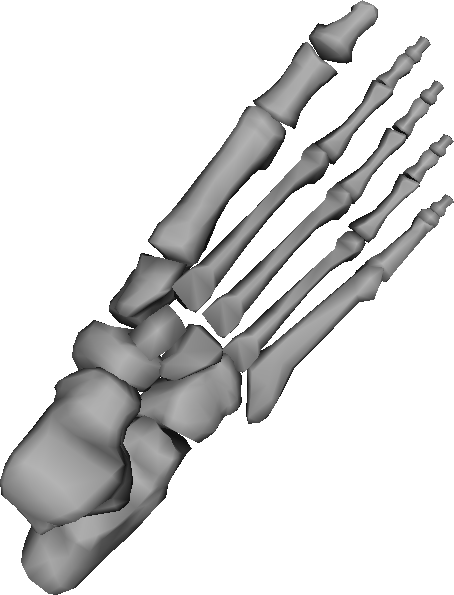
\includegraphics[width=0.45\textwidth]{pictures/image01.png}
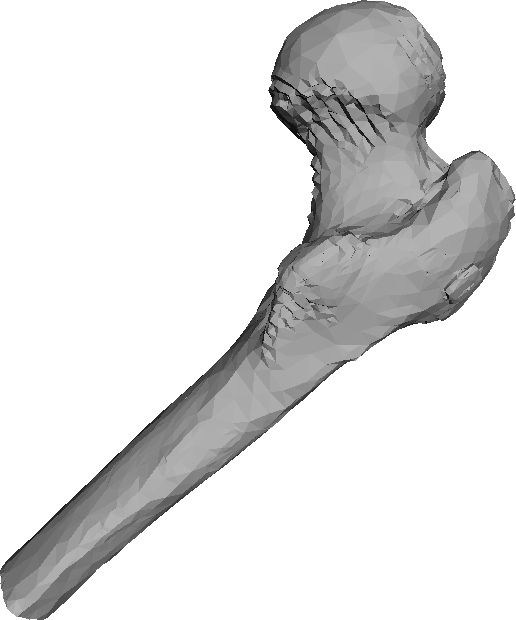
\includegraphics[width=0.45\textwidth]{pictures/image02.png}
\caption{Meshes generated from medical data. Data obtained from the AIM$@$SHAPE Shape Repository \cite{AIMSHAPE}}
\label{fig:example}
\end{figure}


This document is structured as follows. In Chapter~\ref{cha:Previous Work} we present some previous work relevant to our problem. In Chapter~\ref{cha:Proposal} we explain our proposal. In Chapter~\ref{cha:Results} we show our results. Finally, in Chapter~\ref{cha:Conclusion} we present our conclusion and future work.


